\documentclass[12pt,a4paper]{article}
%\usepackage{ctex}
\usepackage{amsmath,amscd,amsbsy,amssymb,latexsym,url,bm,amsthm}
\usepackage{epsfig,graphicx,subfigure}
\usepackage{enumitem,balance}
\usepackage{wrapfig}
\usepackage{mathrsfs, euscript}
\usepackage[usenames]{xcolor}
\usepackage{hyperref}
\usepackage[vlined,ruled,commentsnumbered,linesnumbered]{algorithm2e}
%\usepackage{algorithm}
\usepackage{float}
\usepackage{array}
\usepackage{diagbox}
\usepackage{color}
\usepackage{indentfirst}
\usepackage{fancyhdr}
\usepackage{gensymb}
\usepackage{geometry}
\usepackage{setspace}
\usepackage{aurical}
\usepackage{times}
\usepackage{caption}
\usepackage{fontspec}
\usepackage{booktabs}
\setmainfont{Times New Roman}

\newtheorem{theorem}{Theorem}[section]
\newtheorem{lemma}[theorem]{Lemma}
\newtheorem{proposition}[theorem]{Proposition}
\newtheorem{corollary}[theorem]{Corollary}
\newtheorem{exercise}{Exercise}[section]
\newtheorem*{solution}{Solution}
\theoremstyle{definition}


\renewcommand{\thefootnote}{\fnsymbol{footnote}}

\newcommand{\postscript}[2]
 {\setlength{\epsfxsize}{#2\hsize}
  \centerline{\epsfbox{#1}}}

\renewcommand{\baselinestretch}{1.0}

\setlength{\oddsidemargin}{-0.365in}
\setlength{\evensidemargin}{-0.365in}
\setlength{\topmargin}{-0.3in}
\setlength{\headheight}{0in}
\setlength{\headsep}{0in}
\setlength{\textheight}{10.1in}
\setlength{\textwidth}{7in}
\makeatletter \renewenvironment{proof}[1][Proof] {\par\pushQED{\qed}\normalfont\topsep6\p@\@plus6\p@\relax\trivlist\item[\hskip\labelsep\bfseries#1\@addpunct{.}]\ignorespaces}{\popQED\endtrivlist\@endpefalse} \makeatother
\makeatletter
\renewenvironment{solution}[1][Solution] {\par\pushQED{\qed}\normalfont\topsep6\p@\@plus6\p@\relax\trivlist\item[\hskip\labelsep\bfseries#1\@addpunct{.}]\ignorespaces}{\popQED\endtrivlist\@endpefalse} \makeatother

\begin{document}
\noindent
%==========================================================
\noindent\framebox[\linewidth]{\shortstack[c]{
\Large{\textbf{Report on Homework 1}}\vspace{1mm}\\ 
CS420, Machine Learning, Shikui Tu, Autumn 2017 \vspace{1mm} \\
Zelin Ye 515030910468}}

\vspace{-0.5\baselineskip}
\section{k-means vs GMM}

Basically, k-means employs One-in-K assignment while GMM utilizes soft assignment. It turns out that k-means has bad robust. Therefore, I tend to introduce some of the ideas in GMM into k-means to form a new variant of k-means.

\vspace{0.003\linewidth}
There are two main differences in my variant of k-means algorithm compared with the original:

\begin{itemize}
	\setlength{\itemsep}{0pt}
	\item I introduce parts of the soft assignment into k-means to make it more robust.
	
	\item I affiliate a hyper parameter $Thres$ into original k-means. When the posteriori probablity is large than $Thres$, it can be retained, or it would be 0.
\end{itemize}

The pseudo-codes of my algorithm can refer to Alg. \ref{alg:kmean_vs_GMM}.

\begin{algorithm}[H]
	\SetKwInOut{Input}{input}
	\SetKwInOut{Output}{output}
	\caption{Improvements of k-means}
	\label{alg:kmean_vs_GMM}
	\vspace{0.25\baselineskip}
	
	\Input{The number of clusters $K$}
	\Output{$\pi_{k}, \mu_{k}, \Sigma_{k}, (k=1,2,...,K)$}
	Initialize the means $\mu_{k}$, covariances $\Sigma_{k}$, mixing coefficients $\pi_{k}$ and threshold $Thres$.
	
	Evaluating the initial value of the log likelihood.
	
	\While{the convergence criterion of parameters or log likelihood is not satisfied}{
	
		\textbf{E step.} Evaluate the responsibilities using the current parameter values:
		\BlankLine
		
		\begin{center}
			$\omega \leftarrow \dfrac{\pi_{k}\mathcal{N}(x_{n}|\mu_{k}, \Sigma_{k})}{\sum\limits_{j=1}^{K}\pi_{j}\mathcal{N}(x_{n}|\mu_{j}, \Sigma_{j})}$\quad $,$ \quad
			$\gamma(z_{nk}) \leftarrow \left\{
				\begin{aligned}
					\omega & & {\omega > Thres} \\
					0 & & {\omega \leq Thres}
				\end{aligned}
			\right.$
		\end{center}
		
		\begin{center}
			$z_{n} \leftarrow \dfrac{e^{z_{n_{i}}}}{\sum\limits_{j=1}^{K}e^{z_{n_{j}}}}$
		\end{center}
		
		\textbf{M step.} Re-estimate the parameters using the current responsibilities:
		
		\begin{center}
			$N_{k} \leftarrow \sum\limits_{n=1}^{N}\gamma(z_{nk})$\quad $,$ \quad
			$\mu^{new}_{k} \leftarrow \dfrac{1}{N_{k}}\sum\limits_{n=1}^{N}\gamma(z_{nk})x_{n}$
		\end{center}
		
		\begin{center}
			$\Sigma^{new}_{k} \leftarrow \dfrac{1}{N_{k}}\sum\limits_{n=1}^{N}\gamma(z_{nk})(x_{n}-\mu^{new}_{k})(x_{n}-\mu^{new}_{k})^{T}$
		\end{center}
		
		\begin{center}
			$\pi^{new}_{k} \leftarrow \dfrac{N_{k}}{N}$
		\end{center}
		
		Evaluate the log likelihood:
		
		\begin{center}
			ln $p(X|\mu,\Sigma,\pi) \leftarrow \sum\limits_{k=1}^{K}$ ln$\left\{\sum\limits_{k=1}^{K}\pi_{k}\mathcal{N}(x_{n}|\mu_{k}, \Sigma_{k})\right\}.$
		\end{center}
	}
	\Return $\pi_{k}, \mu_{k}, \Sigma_{k}, (k=1,2,...,K)$\;
\end{algorithm}

With the introduction of probability, my algorithm is somewhat similar to EM algorithm and would be more robust than k-means. Besides, the $Thres$ would eliminate the negligible posteriori probabilities and improve accuracy under the premise of robustness.

Generally speaking, more hyper parameters would result in more tricks, my algorithm is no exception. The choice of $Thres$ may greatly affect the result.

Additionally, my algorithm also encounters the initialization and unknown $K$ problems. But I think such problems do not contradict with my core ideas, and could be resolved by introducing more components (e.g. the idea of RPCL).

\vspace{-1\baselineskip}
\section{k-means vs CL}

\subsection{Comparison between k-means and CL}

\begin{itemize}
	\item \textbf{Similarities}
	
	\begin{enumerate}
		\item They can not estimate the total number of clusters from data.
		
		\item The effects of these two algorithms highly rely on initialization.
		
		\item Both of them have huge potential for expansion to improve their robustness.
		
		\item They consider data in distance framework instead of probability.
	\end{enumerate}
	
	\item \textbf{Differences}
	
	\begin{enumerate}
		\item k-means is a batch learning algorithm while CL belongs to adaptive learning.
		
		\item CL has a hyper parameter $\eta$ to adjust, making the algorithm a little tricky. But k-means has no hyper parameter.
		
		\item k-means would take more time to converge when it comes to large data size. CL avoids this issue by updating the center by one data point each time.
		
		\item Comparing to k-means, CL requires less computing resource (CPU, memory and etc).

		\item The process of k-means is more simple and succinct than CL.
	\end{enumerate}
\end{itemize}

\subsection{Application of RPCL in k-means}

Since k-means can not estimate the total number of clusters from data while RPCL can make extra centers far away to control the number of clusters, I tend to apply the idea of RPCL to \textbf{the initialization of k-means}.

Suppose the initial number of centers is $m$ and the corresponding weight vectors are $v_{i}(i=1,...,m)$. For each center, its output could be defined as:

\begin{equation}
	\centering
	u_{i}\leftarrow \left\{
		\begin{aligned}
			1 & \quad \text{if $u_{i}$ is the winner} \\
			-1 & \quad \text{if $u_{i}$ is the rival} \\
			0 & \quad \text{otherwise}
		\end{aligned},
	\right.
	\label{eqn:1}
\end{equation}

To make the winner approach the center of target cluster faster and keep rival away from it more efficiently, I take the geometric distribution of the data points into consideration. Therefore, a density function for each data point is defined as:

\begin{equation}
	\rho(x_{j}) = \exp[-\sum\limits_{i=1}^{N}\dfrac{d(x_{i}, x_{j})}{\sum\limits_{i=1}^{N}d(x_{1}, x_{j})}], j = 1,2,...,N
\end{equation}
where $d$ denotes the distance function.

Then the adjustment for each weight vector $v_{i}$ can be conducted according to $u_{i}$ and $\rho(x_{j})$:

\begin{equation}
	\centering
	\Delta v_{i} = \left\{
		\begin{aligned}
			\alpha_{i}\rho(x_{j})&(x_{j}-v_{i}) \quad u_{i} = 1 \\
			\beta_{i}\rho(x_{j})&(x_{j}-v_{i}) \quad u_{i} = -1 \\
			& 0 \quad \quad \qquad \text{otherwise}
		\end{aligned},
	\right.
	\label{eqn:4}
\end{equation}
where $\alpha$ and $\beta$ are hyper parameters.

Once the weight vectors converge, I will eliminate negligible ones according to a threshold $T$. Then the number of the remaining centers should be the clusters number $K$, and these centers would locate in 'good' initial positions.

\vspace{0.008\linewidth}
The pseudo-codes of my algorithm can refer to Alg. \ref{alg:RPCL}.

\begin{algorithm}[H]
	\SetKwInOut{Input}{input}
	\SetKwInOut{Output}{output}
	\caption{RPCL in k-means}
	\label{alg:RPCL}
	\vspace{0.25\baselineskip}
	
	\Input{The dataset}
	\Output{The initial centers and corresponding weight vectors}
	Initialize the number of centers $m$ and weight vectors $v_{i}$, threshold $T$, density $\rho(x_{j})$.
	
	\While {the convergence criterion is not satisfied} {
		\For {i = 0 to n}{
			Calculating $u_{i}$ according to Eqn. \ref{eqn:1}.
			
			Adjust the weight vectors of each centers via Eqn. \ref{eqn:4}.
		}
	}
	
	Assign each data point to its closest center.
	
	\For {i = 0 to m} {
		\begin{equation*}
			\eta \leftarrow \dfrac{N_{i}}{N},
		\end{equation*}
		where $N_{i}$ denotes the number of data points in $ith$ center, $N$ is the number of data points in the dataset.
		
		\If {$\eta < T$} {
			Remove center $v_{i}$.
		}
	}

	\Return $v$;
\end{algorithm}

I test this application in a three-cluster dataset generated by myself, and the results of initial centers choice can refer to Fig. \ref{fig:RPCL}.

\begin{figure}[htbp]
	\centering
	\subfigure[Initialization\_1]{
	    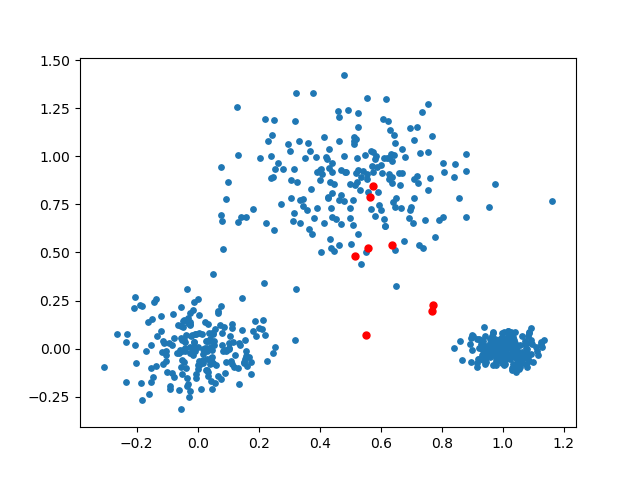
\includegraphics[width=0.23\linewidth]{demo/RPCL_3_1_0.png}
	}
	\subfigure[Result\_1]{
	    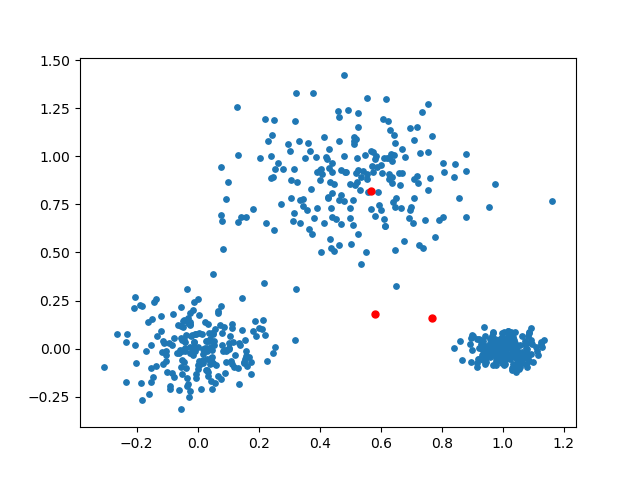
\includegraphics[width=0.23\linewidth]{demo/RPCL_3_2_0.png}
	}
	% % % % % % % % % %
	\subfigure[Initialization\_2]{
	    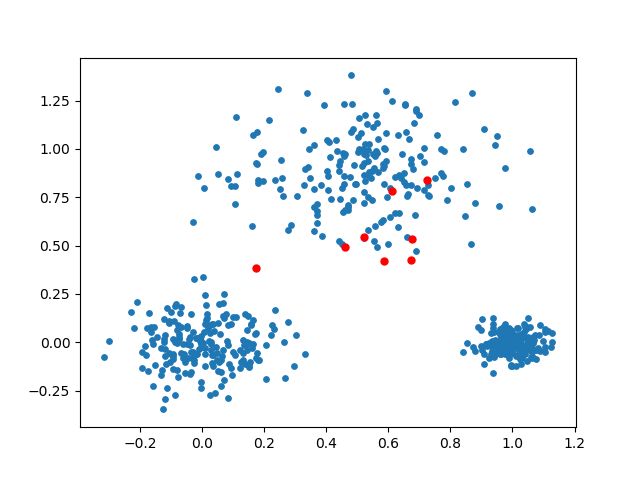
\includegraphics[width=0.23\linewidth]{demo/RPCL_3_1.png}
	}
	\subfigure[Result\_2]{
	    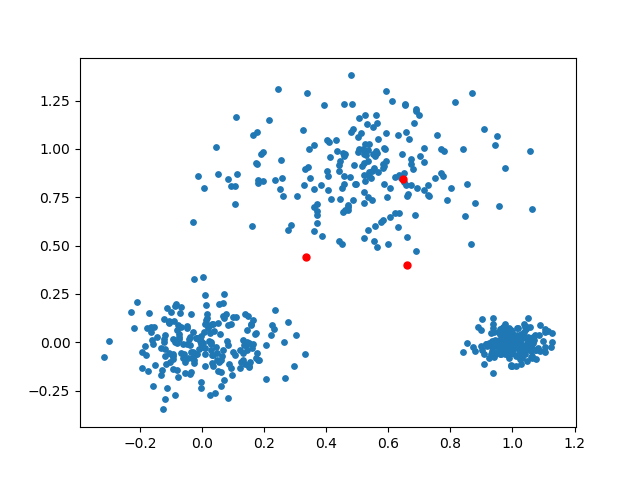
\includegraphics[width=0.23\linewidth]{demo/RPCL_3_2.png}
	}
	\caption{The results of RPCL in kmeans. Blue points denotes data and red points denotes cluster centers.}
	\label{fig:RPCL}
\end{figure}

It turns out that RPCL could determine the number of clusters and even provide a good initialization, which greatly speeds up the process of kmeans.

%\vspace{-1\baselineskip}
\section{Model Selection of GMM}

In this section, I compare model selection performances among BIC, AIC and VBEM by varying the sample sizes and the cluster center distances of the dataset (All the datasets are randomly generated based on GMM).

\subsection{Different Sample Sizes}
\label{sec:1}
In this experiment, I genetate 4 clusters on the four corners of a square, and run BIC, AIC and VBEM with different sample sizes. Then I visualize the result to check their performaces, which are shown in Fig. \ref{fig:sample_comp1}. The corresponding line chart can refer to Fig. \ref{fig:sample_line}.

\begin{figure}[htbp]
	\centering
	\subfigure{
	    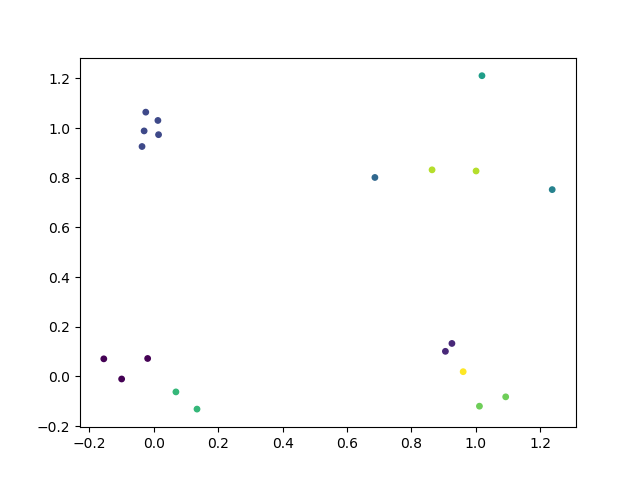
\includegraphics[width=0.18\linewidth]{demo/bic_5_10.png}
	}
	\subfigure{
	    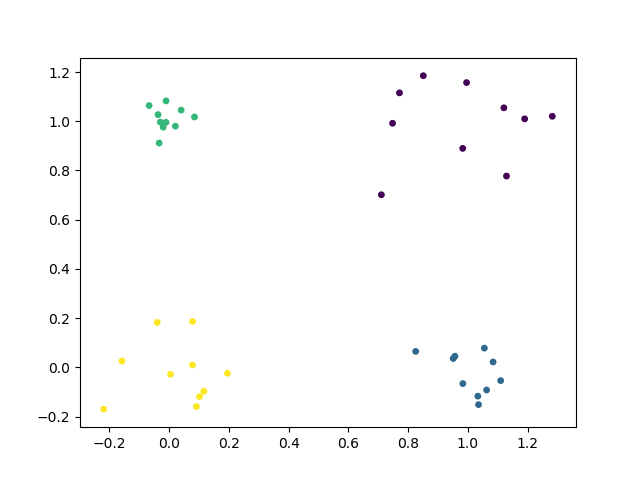
\includegraphics[width=0.18\linewidth]{demo/bic_10_4.png}
	}
	\subfigure{
	    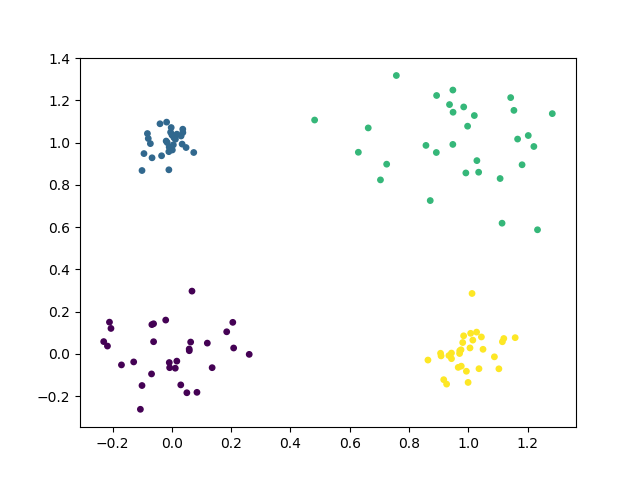
\includegraphics[width=0.18\linewidth]{demo/bic_30_4.png}
	}
	\subfigure{
	    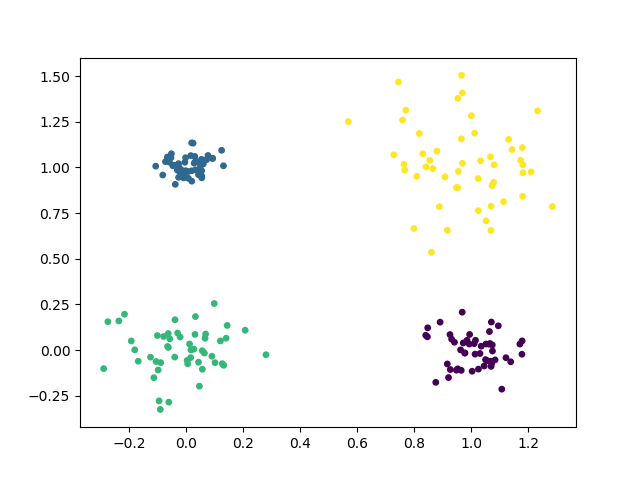
\includegraphics[width=0.18\linewidth]{demo/bic_50_4.png}
	}
	\subfigure{
	    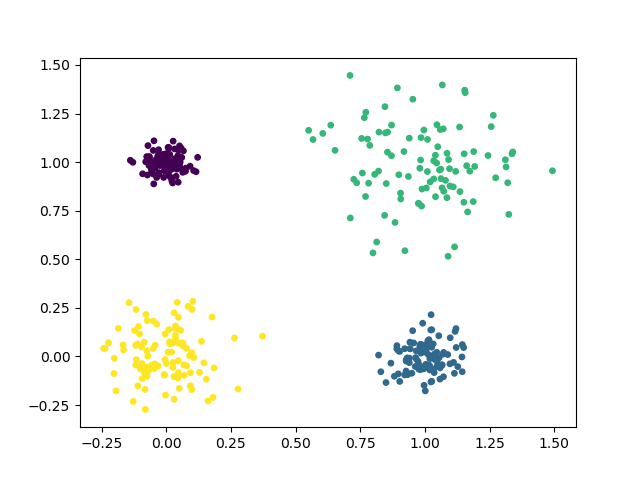
\includegraphics[width=0.18\linewidth]{demo/bic_100_4.png}
	}
	% % % % % % % % % %
	\subfigure{
	    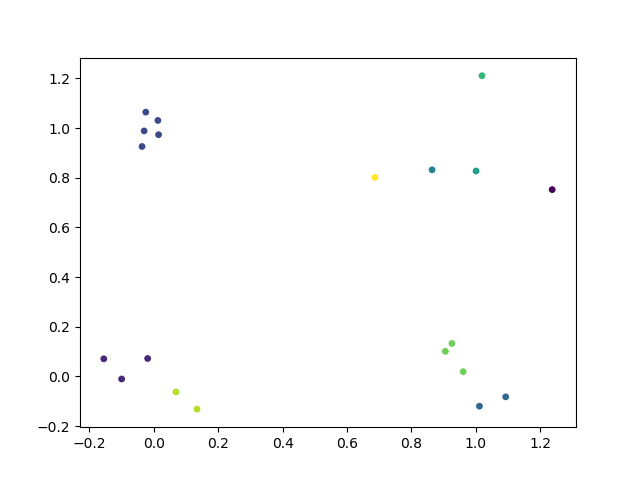
\includegraphics[width=0.18\linewidth]{demo/aic_5_10.png}
	}
	\subfigure{
	    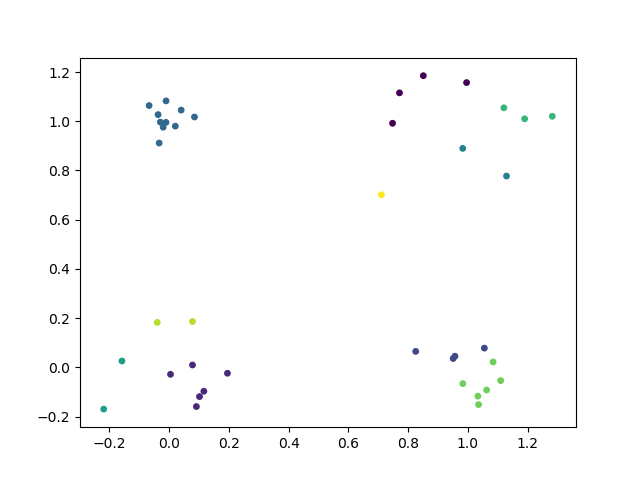
\includegraphics[width=0.18\linewidth]{demo/aic_10_10.png}
	}
	\subfigure{
	    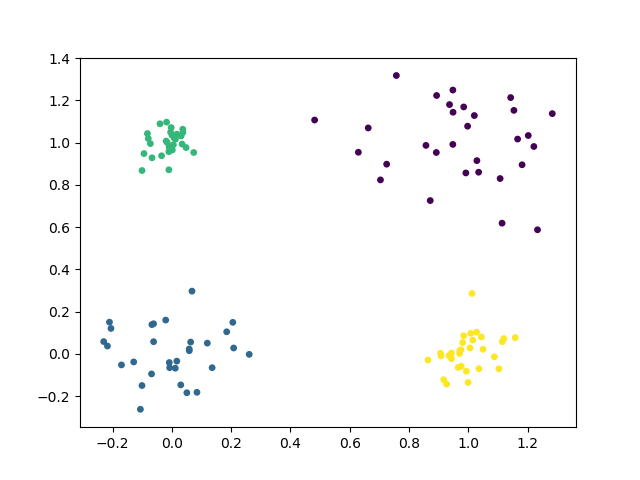
\includegraphics[width=0.18\linewidth]{demo/aic_30_4.png}
	}
	\subfigure{
	    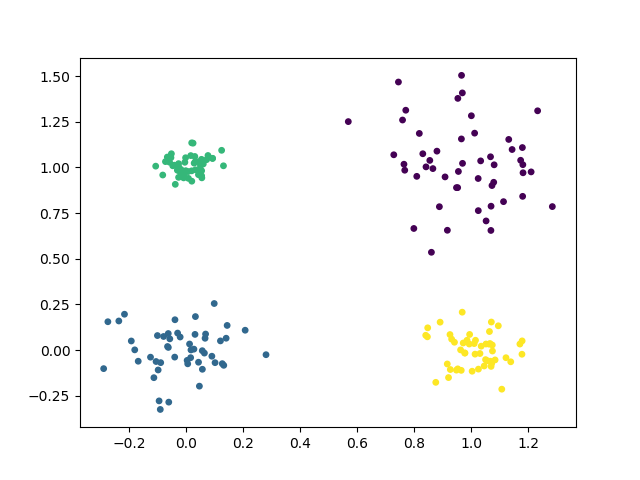
\includegraphics[width=0.18\linewidth]{demo/aic_50_4.png}
	}
	\subfigure{
	    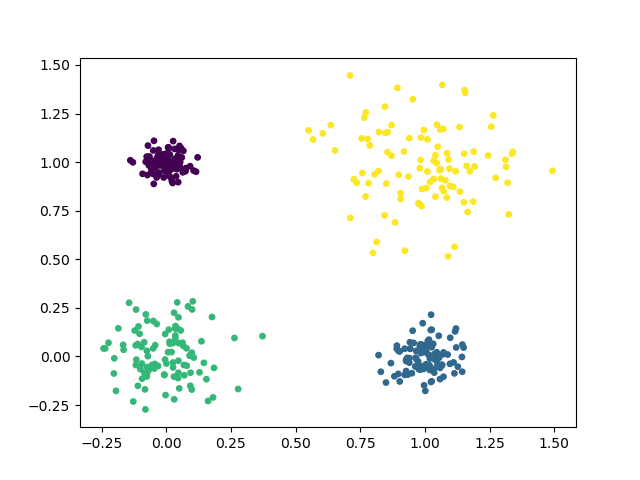
\includegraphics[width=0.18\linewidth]{demo/aic_100_4.png}
	}
	% % % % % % % % % %
	\subfigure{
	    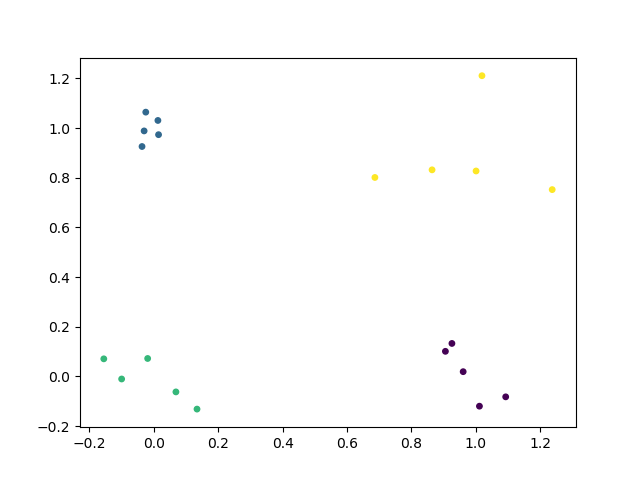
\includegraphics[width=0.18\linewidth]{demo/vbem_5_4.png}
	}
	\subfigure{
	    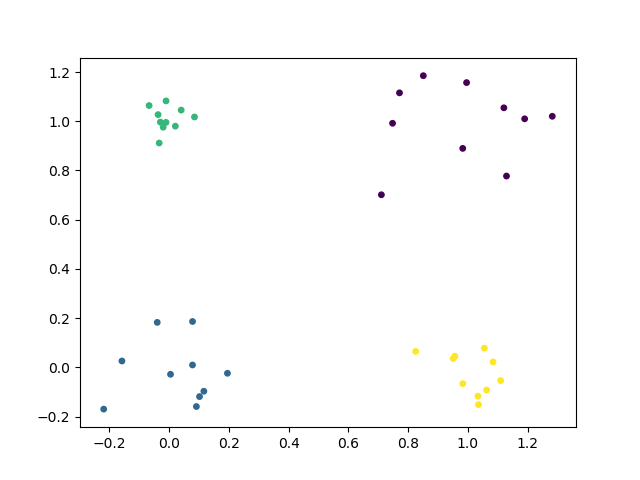
\includegraphics[width=0.18\linewidth]{demo/vbem_10_4.png}
	}
	\subfigure{
	    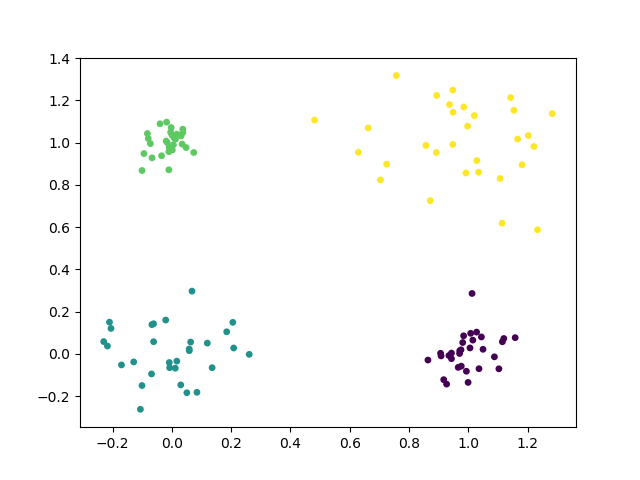
\includegraphics[width=0.18\linewidth]{demo/vbem_30_4.png}
	}
	\subfigure{
	    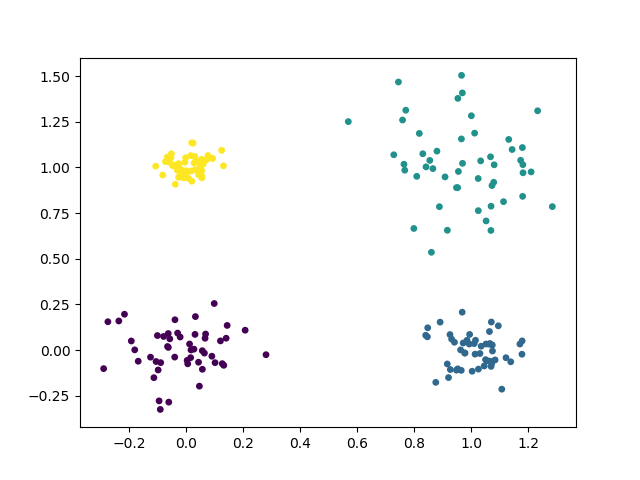
\includegraphics[width=0.18\linewidth]{demo/vbem_50_4.png}
	}
	\subfigure{
	    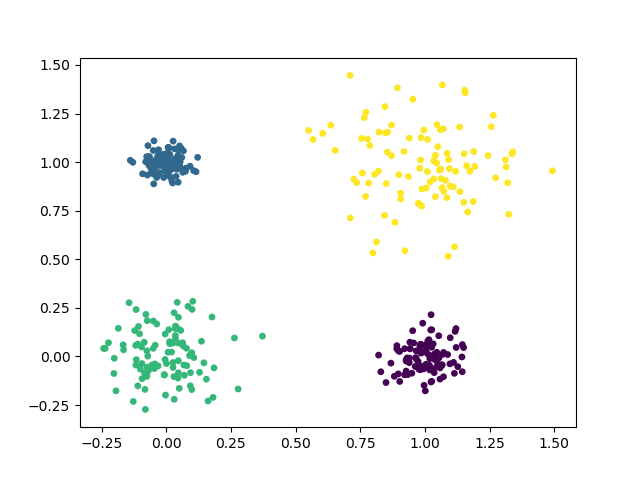
\includegraphics[width=0.18\linewidth]{demo/vbem_100_4.png}
	}
	\caption{The model selection performances of BIC, AIC and VBEM on different sample sizes. Each row from up to bottom denotes BIC, AIC and VBEM respectively. Each column from left to right denotes different sample sizes(5, 10, 30, 50, 100).}
	\label{fig:sample_comp1}
\end{figure}

\begin{figure}[H]
	\centering
	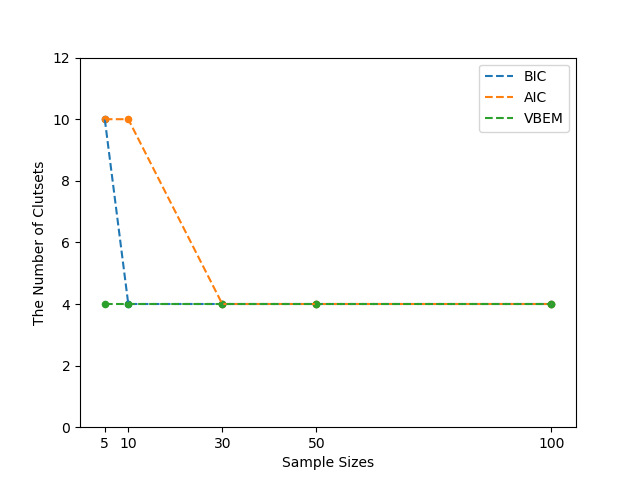
\includegraphics[width=0.5\linewidth]{demo/sample_line.png}
	\caption{The Model Selection Performances of BIC, AIC and VBEM on Different Sample Sizes.}
	\label{fig:sample_line}
\end{figure}

It can be found from the results that all of the three approaches perform well in middle or large sample sizes. When it comes to small sample sizes, BIC and AIC are more likely to  get pool performance while VBEM can prevent such cases. More exactly, BIC outperforms AIC slightly in small sample sizes.

In this experiment, VBEM archieve best clutsering result, BIC is the next and AIC is the worst.

\subsection{Different Distance Among Cluster Centers}
\label{sec:2}

After exploring the effects of sample sizes on the three approaches, I feel curious about how the distance among cluster centers affect their performance.

I generate 3 clusters on the three corners of a  equilateral triangle, reducing the distance among them and visualizing the model selection results in Fig. \ref{fig:dis}.

\begin{figure}[H]
	\centering
	\subfigure[bic-0.3-2]{
	    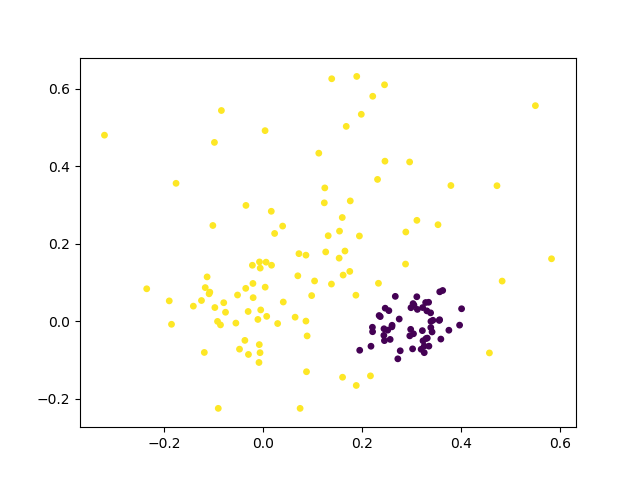
\includegraphics[width=0.23\linewidth]{demo/dis_bic_3_2.png}
	}
	\subfigure[bic-0.7-3]{
	    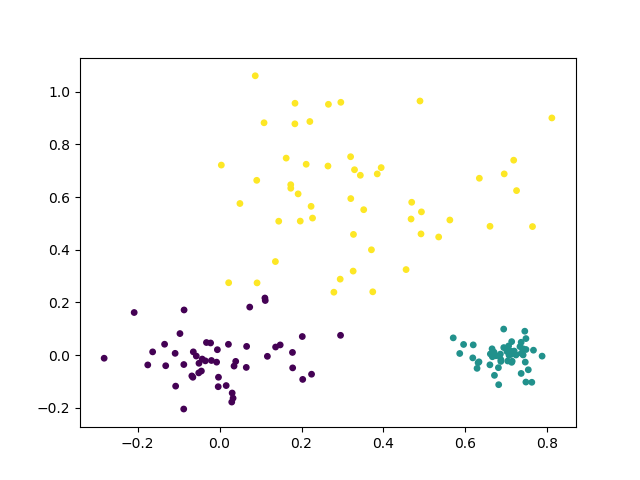
\includegraphics[width=0.23\linewidth]{demo/dis_bic_7_3.png}
	}
	\subfigure[bic-1-3]{
	    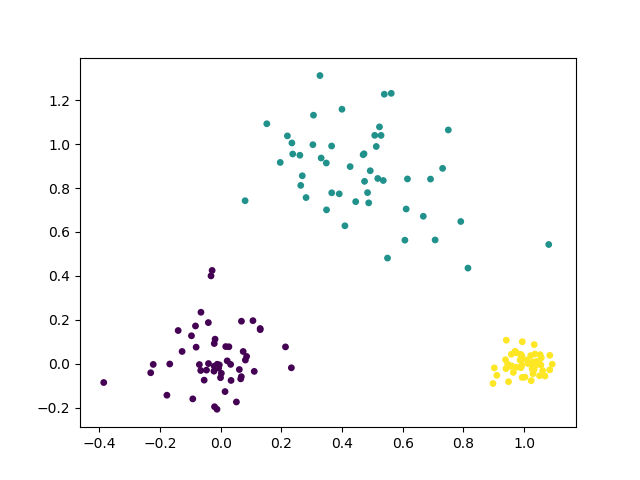
\includegraphics[width=0.23\linewidth]{demo/dis_bic_10_3.png}
	}
	\subfigure[bic-3-3]{
	    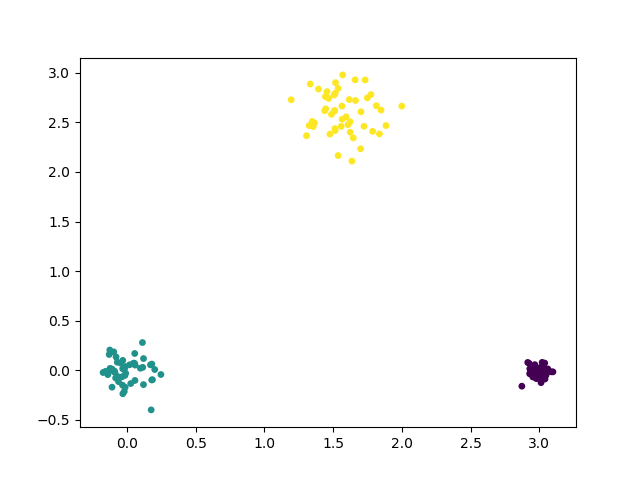
\includegraphics[width=0.23\linewidth]{demo/dis_bic_30_3.png}
	}
	% % % % % % % % % %
	\subfigure[aic-0.3-3]{
	    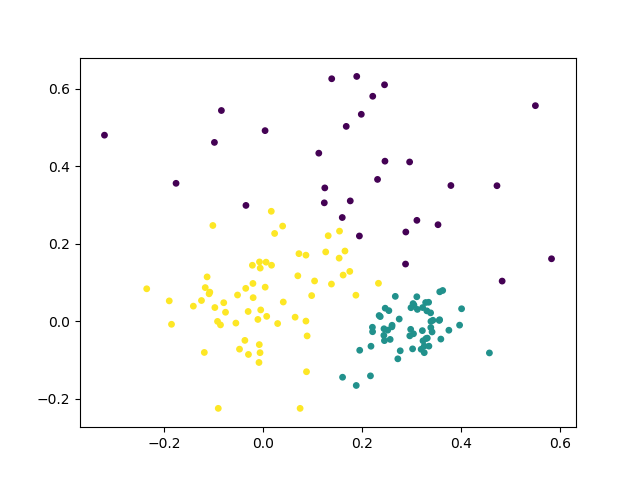
\includegraphics[width=0.23\linewidth]{demo/dis_aic_3_3.png}
	}
	\subfigure[aic-0.7-6]{
	    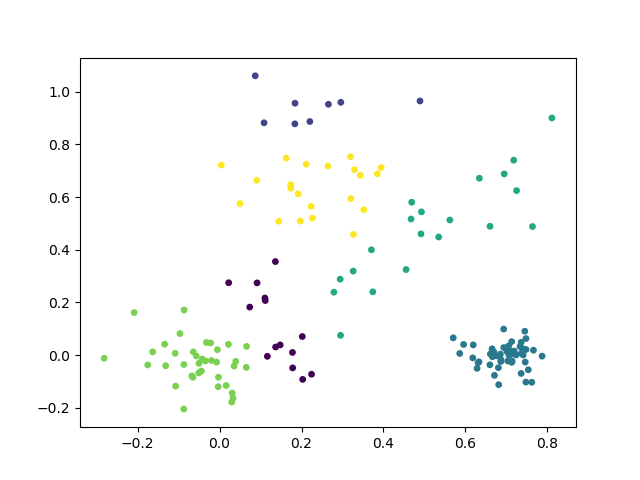
\includegraphics[width=0.23\linewidth]{demo/dis_aic_7_6.png}
	}
	\subfigure[aic-1-10]{
	    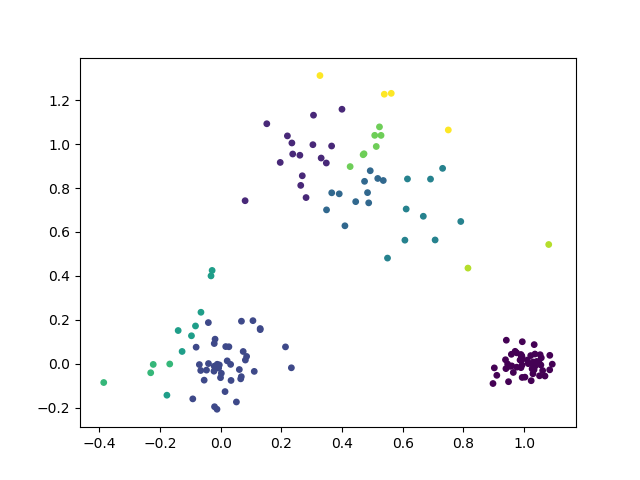
\includegraphics[width=0.23\linewidth]{demo/dis_aic_10_10.png}
	}
	\subfigure[aic-3-9]{
	    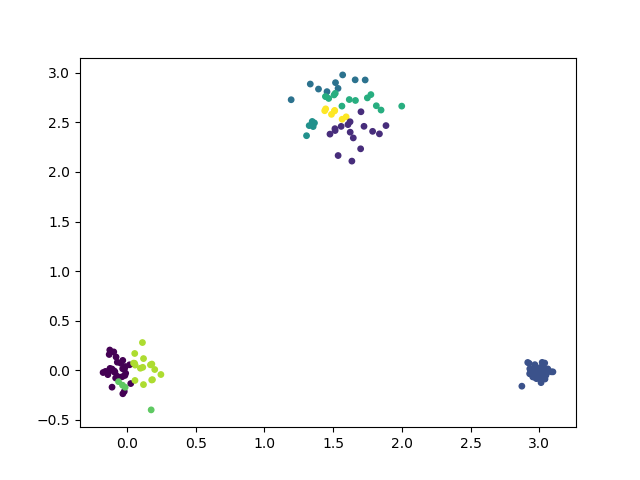
\includegraphics[width=0.23\linewidth]{demo/dis_aic_30_9.png}
	}
	% % % % % % % % % %
	\subfigure[vbem-0.3-3]{
	    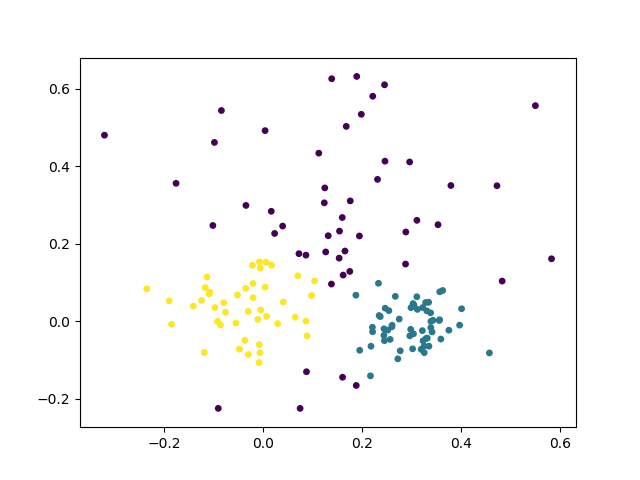
\includegraphics[width=0.23\linewidth]{demo/dis_vbem_3_3.png}
	}
	\subfigure[vbem-0.7-4]{
	    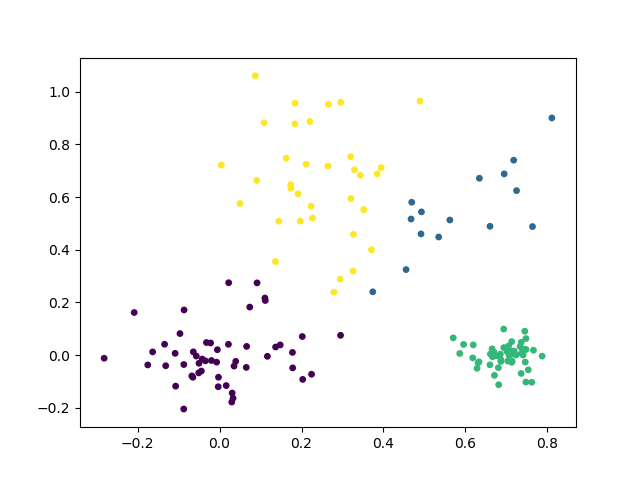
\includegraphics[width=0.23\linewidth]{demo/dis_vbem_7_3.png}
	}
	\subfigure[vbem-1-3]{
	    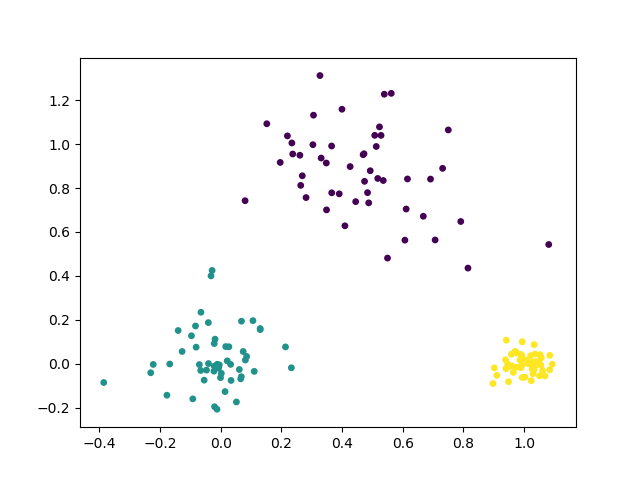
\includegraphics[width=0.23\linewidth]{demo/dis_vbem_10_3.png}
	}
	\subfigure[vbem-3-3]{
	    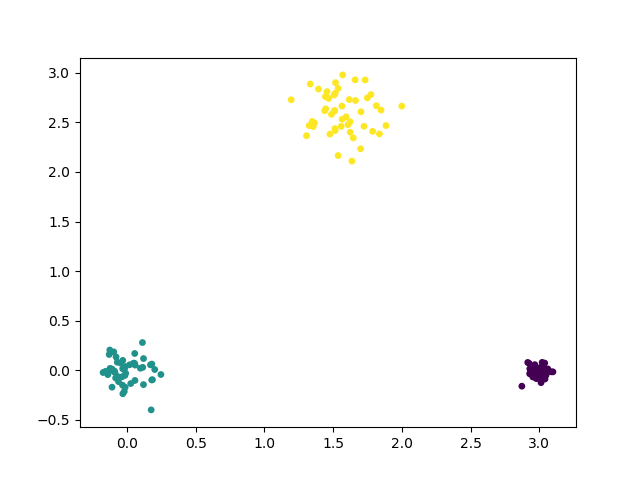
\includegraphics[width=0.23\linewidth]{demo/dis_vbem_30_3.png}
	}
	\caption{The model selection performances of BIC, AIC and VBEM on different cluster center distances. Each row from up to bottom denotes BIC, AIC and VBEM respectively. The two numbers below each figure denote the distance among three cluster centers and the $K$ chosen by corresponding approach respectively.}
	\label{fig:dis}
\end{figure}

As is shown in the results, BIC and VBEM outperform AIC a lot, especially in long distance cases, where AIC tends to choose models having more cluster centers.

\subsection{Discussion \& Conclusion}

In the experiments, I mainly compare the model selection ability of BIC, AIC and VBEM under different sample sizes and cluster center distances. From the results of Sec. \ref{sec:1} and Sec. \ref{sec:2}, VBEM performs best, BIC is just a little bit worse and AIC performs worst.

Actually, though these experiments can reveal their performance to a certain extent, they are only a small portion of comparisons among the three approaches and the results may be variant in other conditions. To be more accurate and comprehensive, more kinds of contrast experiments needed (e.g. different data dimensions, number of clusters).

Ultimately, I want to express my sincere thanks to Prof. Shikui Tu and TA Yajing Chen for their patient guidance and great help in this homework! Thank you!

%========================================================================
\end{document}